\documentclass{article}
\usepackage[utf8]{inputenc}
\usepackage{amsmath}
\usepackage{algorithmicx}
\usepackage{algorithm}
\usepackage{algpseudocode}
\usepackage{indentfirst}
\usepackage{subcaption}
\usepackage{graphicx}

\algnewcommand\algorithmicinput{\textbf{//Input:}}
\algnewcommand\INPUT{\item[\algorithmicinput]}
\algnewcommand\algorithmicoutput{\textbf{//Output:}}
\algnewcommand\OUTPUT{\item[\algorithmicoutput]}

\title{Homework 6}
\author{Lei Zhang}

\begin{document}

\maketitle

\section{Exercieses 6.2 - 1}

\[
C =
\left[
\begin{array}{cccc}
1& 1 & 1 &2 \\
2& 1 &1 &3\\
1& -1 &3&8\\
\end{array}
\right] row 2 - 2 row 1, row 3- row 1
\]

\[
C =
\left[
\begin{array}{cccc}
1& 1 & 1 &2 \\
0& -1 &-1 &-1\\
0& -2 &2& 6\\
\end{array}
\right] row 3 - 2 row 2
\]

\[
C =
\left[
\begin{array}{cccc}
1& 1 & 1 &2 \\
0& -1 &-1 &-1\\
0& 0 & 4& 8\\
\end{array}
\right]
\]

Now we can obtain the solution by back substituations:

$x_3 = 8/4 = 2, x_2 = (-1 + x_3)/(-1) = -1, x_1 = 2 - x_2 - x_3 = 1$

\section{Exercieses 6.2 - 4}

The final answer is correct. The derivation is almost correct except the last step. In the last step, $S(n)_1, S(n)_2,$ and $ S(n)_3$ should not be added wholly. They should be added up for their detailed expressions.

\section{Exercieses 6.4 - 1}


\subsection*{a. }
\graphicspath{{./Figures/}}


\begin{figure}[H]
  \begin{tabular}{cc}
    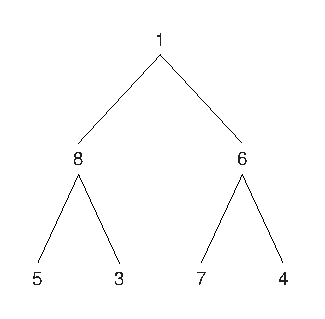
\includegraphics[width=50mm]{1}&
    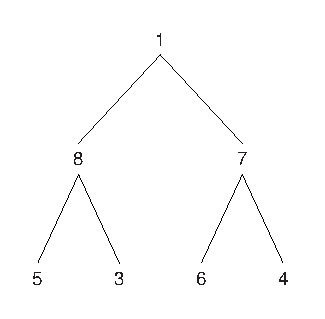
\includegraphics[width=50mm]{2}
    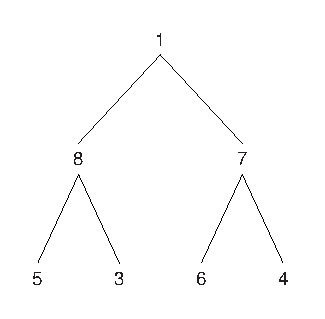
\includegraphics[width=50mm]{3}\\
    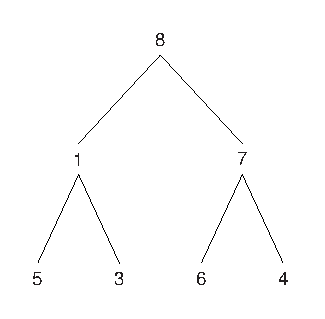
\includegraphics[width=50mm]{4}&
    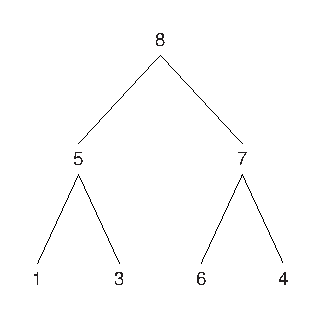
\includegraphics[width=50mm]{5}\\
  \end{tabular}
\end{figure}


\subsection*{b. }

1

1 8

8 1 6

8 1 6 5

8 5 6 1 3

8 5 6 1 3 7

8 5 7 1 3 6 4


\subsection*{c. }

No. It's not. They can yield different heaps for same input, which are both correct.

\section{Exercieses 6.5 - 1}
\begin{align*}
C(n) &= \sum_{i=1}^n(\sum_{j=1}^i(1+1)) \\
&= \sum_{i=0}^n(i+1)\\
&= \frac{n(n+1)}{2} + (n+1)\\
&= \frac{(n+1)(n+2)}{2} \in \theta(n^2)
\end{align*}

\section{Exercieses 6.5 - 4}

\subsection*{a}

\begin{tabular}{cccccc}
\hline
coefficients & 3 & -1 & 0 & 2 & 5\\
x = -2 & 3 & (-2)$\times$ 3-1=-7 & (-2)$\times$ (-7)=14 & (-2)$\times$ 14+2=-26 &(-2)$\times$ (-26)+5=57\\
\hline
\end{tabular}

\subsection*{b}

The quotient is $3x^3 - 7x^2 + 14x -26$, the remainder is $57$.

\end{document}
